%%%%%%%%%%%%%%%%%%%%%%%%%%%%%%%%%%%%%%%%%
% Lachaise Assignment
% LaTeX Template
% Version 1.0 (26/6/2018)
%
% This template originates from:
% http://www.LaTeXTemplates.com
%
% Authors:
% Marion Lachaise & François Févotte
% Vel (vel@LaTeXTemplates.com)
%
% License:
% CC BY-NC-SA 3.0 (http://creativecommons.org/licenses/by-nc-sa/3.0/)
% 
%%%%%%%%%%%%%%%%%%%%%%%%%%%%%%%%%%%%%%%%%

%----------------------------------------------------------------------------------------
%	PACKAGES AND OTHER DOCUMENT CONFIGURATIONS
%----------------------------------------------------------------------------------------

\documentclass{article}

\usepackage{listings}
\usepackage{graphicx}
\usepackage{enumitem}
%\graphicspath{{imgs/}}

%%%%%%%%%%%%%%%%%%%%%%%%%%%%%%%%%%%%%%%%%
% Lachaise Assignment
% Structure Specification File
% Version 1.0 (26/6/2018)
%
% This template originates from:
% http://www.LaTeXTemplates.com
%
% Authors:
% Marion Lachaise & François Févotte
% Vel (vel@LaTeXTemplates.com)
%
% License:
% CC BY-NC-SA 3.0 (http://creativecommons.org/licenses/by-nc-sa/3.0/)
% 
%%%%%%%%%%%%%%%%%%%%%%%%%%%%%%%%%%%%%%%%%

%----------------------------------------------------------------------------------------
%	PACKAGES AND OTHER DOCUMENT CONFIGURATIONS
%----------------------------------------------------------------------------------------

\usepackage{amsmath,amsfonts,stmaryrd,amssymb} % Math packages

\usepackage{enumerate} % Custom item numbers for enumerations

\usepackage[ruled]{algorithm2e} % Algorithms

\usepackage[framemethod=tikz]{mdframed} % Allows defining custom boxed/framed environments

\usepackage{listings} % File listings, with syntax highlighting
\lstset{
	basicstyle=\ttfamily, % Typeset listings in monospace font
}

%----------------------------------------------------------------------------------------
%	DOCUMENT MARGINS
%----------------------------------------------------------------------------------------

\usepackage{geometry} % Required for adjusting page dimensions and margins

\geometry{
	paper=a4paper, % Paper size, change to letterpaper for US letter size
	top=2.5cm, % Top margin
	bottom=3cm, % Bottom margin
	left=2.5cm, % Left margin
	right=2.5cm, % Right margin
	headheight=14pt, % Header height
	footskip=1.5cm, % Space from the bottom margin to the baseline of the footer
	headsep=1.2cm, % Space from the top margin to the baseline of the header
	%showframe, % Uncomment to show how the type block is set on the page
}

%----------------------------------------------------------------------------------------
%	FONTS
%----------------------------------------------------------------------------------------

\usepackage[utf8]{inputenc} % Required for inputting international characters
\usepackage[T1]{fontenc} % Output font encoding for international characters

\usepackage{XCharter} % Use the XCharter fonts

%----------------------------------------------------------------------------------------
%	COMMAND LINE ENVIRONMENT
%----------------------------------------------------------------------------------------

% Usage:
% \begin{commandline}
%	\begin{verbatim}
%		$ ls
%		
%		Applications	Desktop	...
%	\end{verbatim}
% \end{commandline}

\mdfdefinestyle{commandline}{
	leftmargin=10pt,
	rightmargin=10pt,
	innerleftmargin=15pt,
	middlelinecolor=black!50!white,
	middlelinewidth=2pt,
	frametitlerule=false,
	backgroundcolor=black!5!white,
	frametitle={Command Line},
	frametitlefont={\normalfont\sffamily\color{white}\hspace{-1em}},
	frametitlebackgroundcolor=black!50!white,
	nobreak,
}

% Define a custom environment for command-line snapshots
\newenvironment{commandline}{
	\medskip
	\begin{mdframed}[style=commandline]
}{
	\end{mdframed}
	\medskip
}

%----------------------------------------------------------------------------------------
%	FILE CONTENTS ENVIRONMENT
%----------------------------------------------------------------------------------------

% Usage:
% \begin{file}[optional filename, defaults to "File"]
%	File contents, for example, with a listings environment
% \end{file}

\mdfdefinestyle{file}{
	innertopmargin=1.6\baselineskip,
	innerbottommargin=0.8\baselineskip,
	topline=false, bottomline=false,
	leftline=false, rightline=false,
	leftmargin=2cm,
	rightmargin=2cm,
	singleextra={%
		\draw[fill=black!10!white](P)++(0,-1.2em)rectangle(P-|O);
		\node[anchor=north west]
		at(P-|O){\ttfamily\mdfilename};
		%
		\def\l{3em}
		\draw(O-|P)++(-\l,0)--++(\l,\l)--(P)--(P-|O)--(O)--cycle;
		\draw(O-|P)++(-\l,0)--++(0,\l)--++(\l,0);
	},
	nobreak,
}

% Define a custom environment for file contents
\newenvironment{file}[1][File]{ % Set the default filename to "File"
	\medskip
	\newcommand{\mdfilename}{#1}
	\begin{mdframed}[style=file]
}{
	\end{mdframed}
	\medskip
}

%----------------------------------------------------------------------------------------
%	NUMBERED QUESTIONS ENVIRONMENT
%----------------------------------------------------------------------------------------

% Usage:
% \begin{question}[optional title]
%	Question contents
% \end{question}

\mdfdefinestyle{question}{
	innertopmargin=1.2\baselineskip,
	innerbottommargin=0.8\baselineskip,
	roundcorner=5pt,
	nobreak,
	singleextra={%
		\draw(P-|O)node[xshift=1em,anchor=west,fill=white,draw,rounded corners=5pt]{%
		Question \theQuestion\questionTitle};
	},
}

\newcounter{Question} % Stores the current question number that gets iterated with each new question

% Define a custom environment for numbered questions
\newenvironment{question}[1][\unskip]{
	\bigskip
	\stepcounter{Question}
	\newcommand{\questionTitle}{~#1}
	\begin{mdframed}[style=question]
}{
	\end{mdframed}
	\medskip
}

%----------------------------------------------------------------------------------------
%	WARNING TEXT ENVIRONMENT
%----------------------------------------------------------------------------------------

% Usage:
% \begin{warn}[optional title, defaults to "Warning:"]
%	Contents
% \end{warn}

\mdfdefinestyle{warning}{
	topline=false, bottomline=false,
	leftline=false, rightline=false,
	nobreak,
	singleextra={%
		\draw(P-|O)++(-0.5em,0)node(tmp1){};
		\draw(P-|O)++(0.5em,0)node(tmp2){};
		\fill[black,rotate around={45:(P-|O)}](tmp1)rectangle(tmp2);
		\node at(P-|O){\color{white}\scriptsize\bf !};
		\draw[very thick](P-|O)++(0,-1em)--(O);%--(O-|P);
	}
}

% Define a custom environment for warning text
\newenvironment{warn}[1][Warning:]{ % Set the default warning to "Warning:"
	\medskip
	\begin{mdframed}[style=warning]
		\noindent{\textbf{#1}}
}{
	\end{mdframed}
}

%----------------------------------------------------------------------------------------
%	INFORMATION ENVIRONMENT
%----------------------------------------------------------------------------------------

% Usage:
% \begin{info}[optional title, defaults to "Info:"]
% 	contents
% 	\end{info}

\mdfdefinestyle{info}{%
	topline=false, bottomline=false,
	leftline=false, rightline=false,
	nobreak,
	singleextra={%
		\fill[black](P-|O)circle[radius=0.4em];
		\node at(P-|O){\color{white}\scriptsize\bf i};
		\draw[very thick](P-|O)++(0,-0.8em)--(O);%--(O-|P);
	}
}

% Define a custom environment for information
\newenvironment{info}[1][Info:]{ % Set the default title to "Info:"
	\medskip
	\begin{mdframed}[style=info]
		\noindent{\textbf{#1}}
}{
	\end{mdframed}
}
 % Include the file specifying the document structure and custom commands

%----------------------------------------------------------------------------------------
%	ASSIGNMENT INFORMATION
%----------------------------------------------------------------------------------------

\title{Advanced Machine Learning: Assignment \#1} % Title of the assignment

\author{Fabrizio D'Intinosante} % Author name and email address

\date{Università degli Studi di Milano Bicocca --- \today} % University, school and/or department name(s) and a date

%----------------------------------------------------------------------------------------

\begin{document}

\maketitle % Print the title

%----------------------------------------------------------------------------------------
%	INTRODUCTION
%----------------------------------------------------------------------------------------

\section*{Introduzione} % Unnumbered section

%\lstset{language=Python}
%\lstset{frame=lines}
%\lstset{caption={Insert code directly in your document}}
%\lstset{label={lst:code_direct}}
%\lstset{basicstyle=\footnotesize}
%\begin{lstlisting}
%from brg.datastructures import Mesh
 
%mesh = Mesh.from_obj('faces.obj')
%mesh.draw()
%\end{lstlisting}
 
Il dataset contiene informazioni riguardo le inadempienze di pagamento, variabili demografiche, dati di credito, storico dei pagamenti ed estratti conto di possessori di carte di credito di Taiwan da Aprile 2005 a Settembre dello stesso anno, distribuite su \textbf{24 colonne} e \textbf{27000 righe}. 
L'obiettivo è quello di predire le inadempienze di pagamento attraverso l'utilizzo di una \textit{neural network}.

\section{Esplorazione e preprocessing} % Numbered section

Come primo passaggio si è provveduto ad esplorare il \textit{dataset}, le distribuzioni delle variabili esplicative e quella della variabile obiettivo. Come si è potuto osservare tramite visualizzazione la variabile obiettivo presenta un forte sbilanciamento.
%Come si vede in fig.~\ref{fig: y} la variabile obiettivo \textit{default.payment.next.month} presenta un forte sbilanciamento.

%\begin{figure}[h!]
%\centering	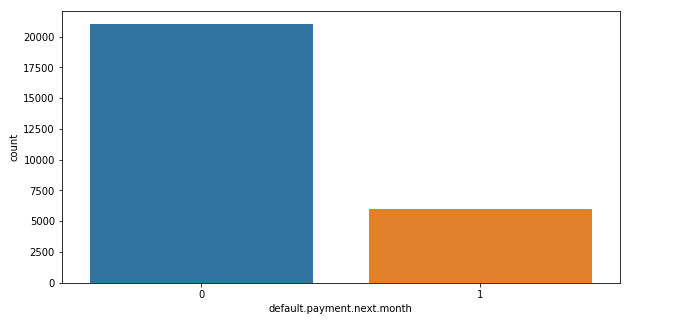
\includegraphics[scale=0.7]{imgs/ydistribution.png}
%	\caption{\label{fig: y} Panoramica sullo sbilanciamento di Y}
%\end{figure}

Per questa ragione si è deciso di procedere alla realizzazione di tre modelli NN:
\begin{itemize}[noitemsep]
\item un modello semplice, che tiene conto dello sbilanciamento solo attraverso l'aggiustamento dei pesi;
\item un modello addestrato su dati sottoposti ad \textit{oversampling} (SMOTE);
\item un modello addestrato su dati sottoposti ad \textit{undersampling}.
\end{itemize}

Le \textit{features} disponibili sono state innanzitutto suddivise in \textit{features} numeriche e categoriche per poter distinguere la strategia di \textit{preprocessing} a loro applicata: mentre infatti per le prime si è deciso di procedere con una semplice standardizzazione (processo che porta la media $\mu = 0$ e la varianza $\sigma^2 = 1$ delle \textit{features}), per le variabili qualitative, in questo caso tutte nominali, si è preferito procedere con la strategia \textit{One-hot encoding} (OHE), ovvero ridurre ogni livello delle variabili ad una \textit{dummy}.

\begin{warn}[NB:]
Durante la creazione delle \textit{dummy} si è proceduto ad eliminare il primo livello di ognuna, così da evitare di incorrere in problemi di multicollinearità.
\end{warn}

Una volta applicate le tecniche di \textit{preprocessing} su entrambi i gruppi di covariate si è proceduto a riunificarle in un unico \textit{numpy array} concatenandole. Successivamente per tutti e tre i modelli i dati sono stati suddivisi in \textit{training set} e \textit{validation set} con una proporzione di 80\% e 20\% (fatta eccezione per il modello con dati trattati con l'\textit{undersampling} per cui si è utilizzata una proporzione 90\% e 10\% per evitare che dopo l'\textit{undersampling} il \textit{training set} risultasse inferiore al \textit{validation set}. 
Il \textit{validation set} oltre ad esser stato utilizzato per l'ottimizzazione degli iperparametri, restando al di fuori del processo di \textit{training} è stato utilizzato anche per la valutazione complessiva del modello attraverso \textit{classification report}.

\begin{warn}[NB:]
Per il secondo ed il terzo modello, ovvero quelli trainati con dati sottoposti ad \textit{oversampling} e \textit{undersapling}, queste tecniche sono state applicate successivamente alla suddivisione tra \textit{training set} e \textit{validation set} così da permettere al modello di apprendere a generalizzare al meglio i dati.
\end{warn}
%------------------------------------------------

\section{Modelli}
Come detto in precedenza i modelli realizzati sono tre: un modello con \textit{balancing} attraverso i pesi, uno con trattamento dei dati attraverso \textit{oversampling} ed un ultimo con trattamento dei dati tramite \textit{undersampling}.
Tutti e tre i modelli condividono tutti gli iperparametri fatta eccezione per il valore di \textit{rate} dei \textit{dropout layer}:
\begin{itemize}[noitemsep]
\item 100 epoche;
\item tre \textit{hidden layers} in ordine da 32, 16 e 16 neuroni. 
Il numero di \textit{layer} e di neuroni è stato scelto dopo aver effettuato diverse prove ed aver verificato che fosse un buon compromesso per non complicare inutilmente il modello implementando però il suo potere predittivo;
\item \textit{activation function hidden layers: }ReLU. 
Scelta standard, si è rivelata la più adeguata;
\item \textit{activation function output layer: Sigmoid}. 
Trattandosi di una classificazione binaria si è trattato di una scelta obbligata considerando che il vettore y è stato mantenuto in forma dummy e non convertito in forma one-hot per cui sarebbe stato necessario utilizzare una \textit{Softmax};
\item pesi personalizzati per unbalancing (utili solo per il primo modello, per gli altri risultano inutili avendo effettuato balancing a priori sui dati tramite \textit{under/oversampling}. 
Per bilanciare lo sbilanciamento della variabile y i pesi così definiti assegnano, nella \textit{loss function} un maggiore peso alla classe sottorappresentata così da bilanciare l'effetto.)
\item \textit{optimizer: }adam. 
Anche questa una scelta piuttosto standard, ottiene buone prestazioni essendo un algoritmo di ottimizzazione adattivo;
\item \textit{loss function: binary\_crossentropy}.
Scelta obbligata trattandosi di stimare valori [0,1];
\item \textit{regularization: }tre \textit{dropout layers} ed \textit{early stopping} con una \textit{patience} di 20.
I rate dei \textit{dropout layers} sono molto piccoli o addirittura azzerati a seconda del modello ma sono stati comunque implementati per poter testare meglio i diversi iperparametri della rete. 
L'unione con l'\textit{early stopping} è stata fatta per scongiurare il rischio di overfitting del modelli.
\end{itemize}
\subsection{Valutazione dei modelli}
Come si vede in fig.~\ref{fig: model1} il modello bilanciato attraverso i pesi è il migliore per valore di \textit{accuracy} ed \textit{weighted avg f1-score}. 
\begin{figure}%[!h]
\centering	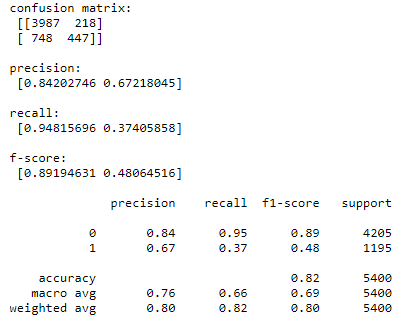
\includegraphics[width=80mm, height=50mm]{imgs/cr_model1.png}
	\caption{\label{fig: model1} \textit{classification report} del modello 1}
\end{figure}
%\newpage
Il modello con dati trattati attraverso \textit{oversampling} invece, il cui \textit{classification report} è presentato in fig.~\ref{fig: model2}, presenta prestazioni inferiori anche se la \textit{f1-score measure} della classe di y meno rappresentata risulta migliore rispetto al modello precedente.
\begin{figure}%[!h]
\centering	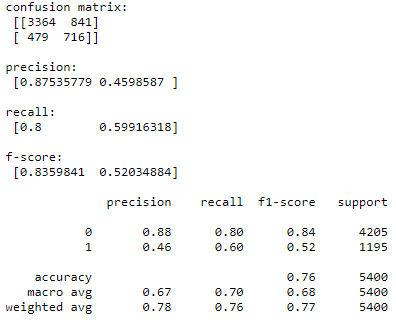
\includegraphics[width=80mm, height=50mm]{imgs/cr_model2.png}
	\caption{\label{fig: model2} \textit{classification report} del modello 2 (oversampling)}
\end{figure}
Il modello con dati trattati invece tramite \textit{undersampling}, presentato in fig.~\ref{fig: model3} risulta tendenzialmente migliore rispetto a quello con dati trattati con \textit{oversampling}, ma comunque inferiori rispetto al primo modello.
\begin{figure}%[!h]
\centering	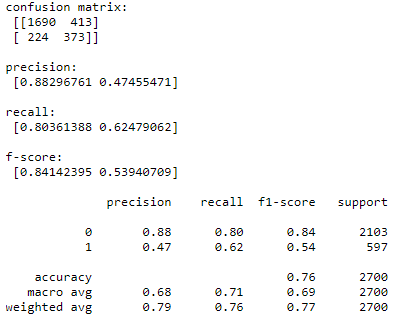
\includegraphics[width=80mm, height=50mm]{imgs/cr_model3.png}
	\caption{\label{fig: model3} \textit{classification report} del modello 3 (undersampling)}
\end{figure}

%----------------------------------------------------------------------------------------
\section{Conclusioni}
In conclusione, si può affermare che il modello vincitore risulti essere quello presentato in fig.~\ref{fig: model1}, ovvero il modello con dati non corretti rispetto all'\textit{unbalancing} presente nella variabile obiettivo y, ma che tratta questo elemento attraverso la correzione dei pesi da sottomettere alla \textit{loss function} così da considerare in modi distinti le osservazioni classificate come 0 e quelle classificate come 1.
%------------------------------------------------------------------------------------------------------------
\end{document}
